\section{Проброс устройств}
\subsection{VPN}

Технология VPN\footnote{VPN (англ. Virtual Private Network) "--- обобщенное название технологий, позволяющих обеспечить одно или несколько сетевых соединений поверх другой сети (например, Интернет)} позволяет устанавливать безопасное сетевое соединение между компьютерами.
Для того чтобы VPN работала в контейнере, необходимо разрешить использование TUN/TAP устройств для контейнера.
\begin{figure}[ht]
    \centering
	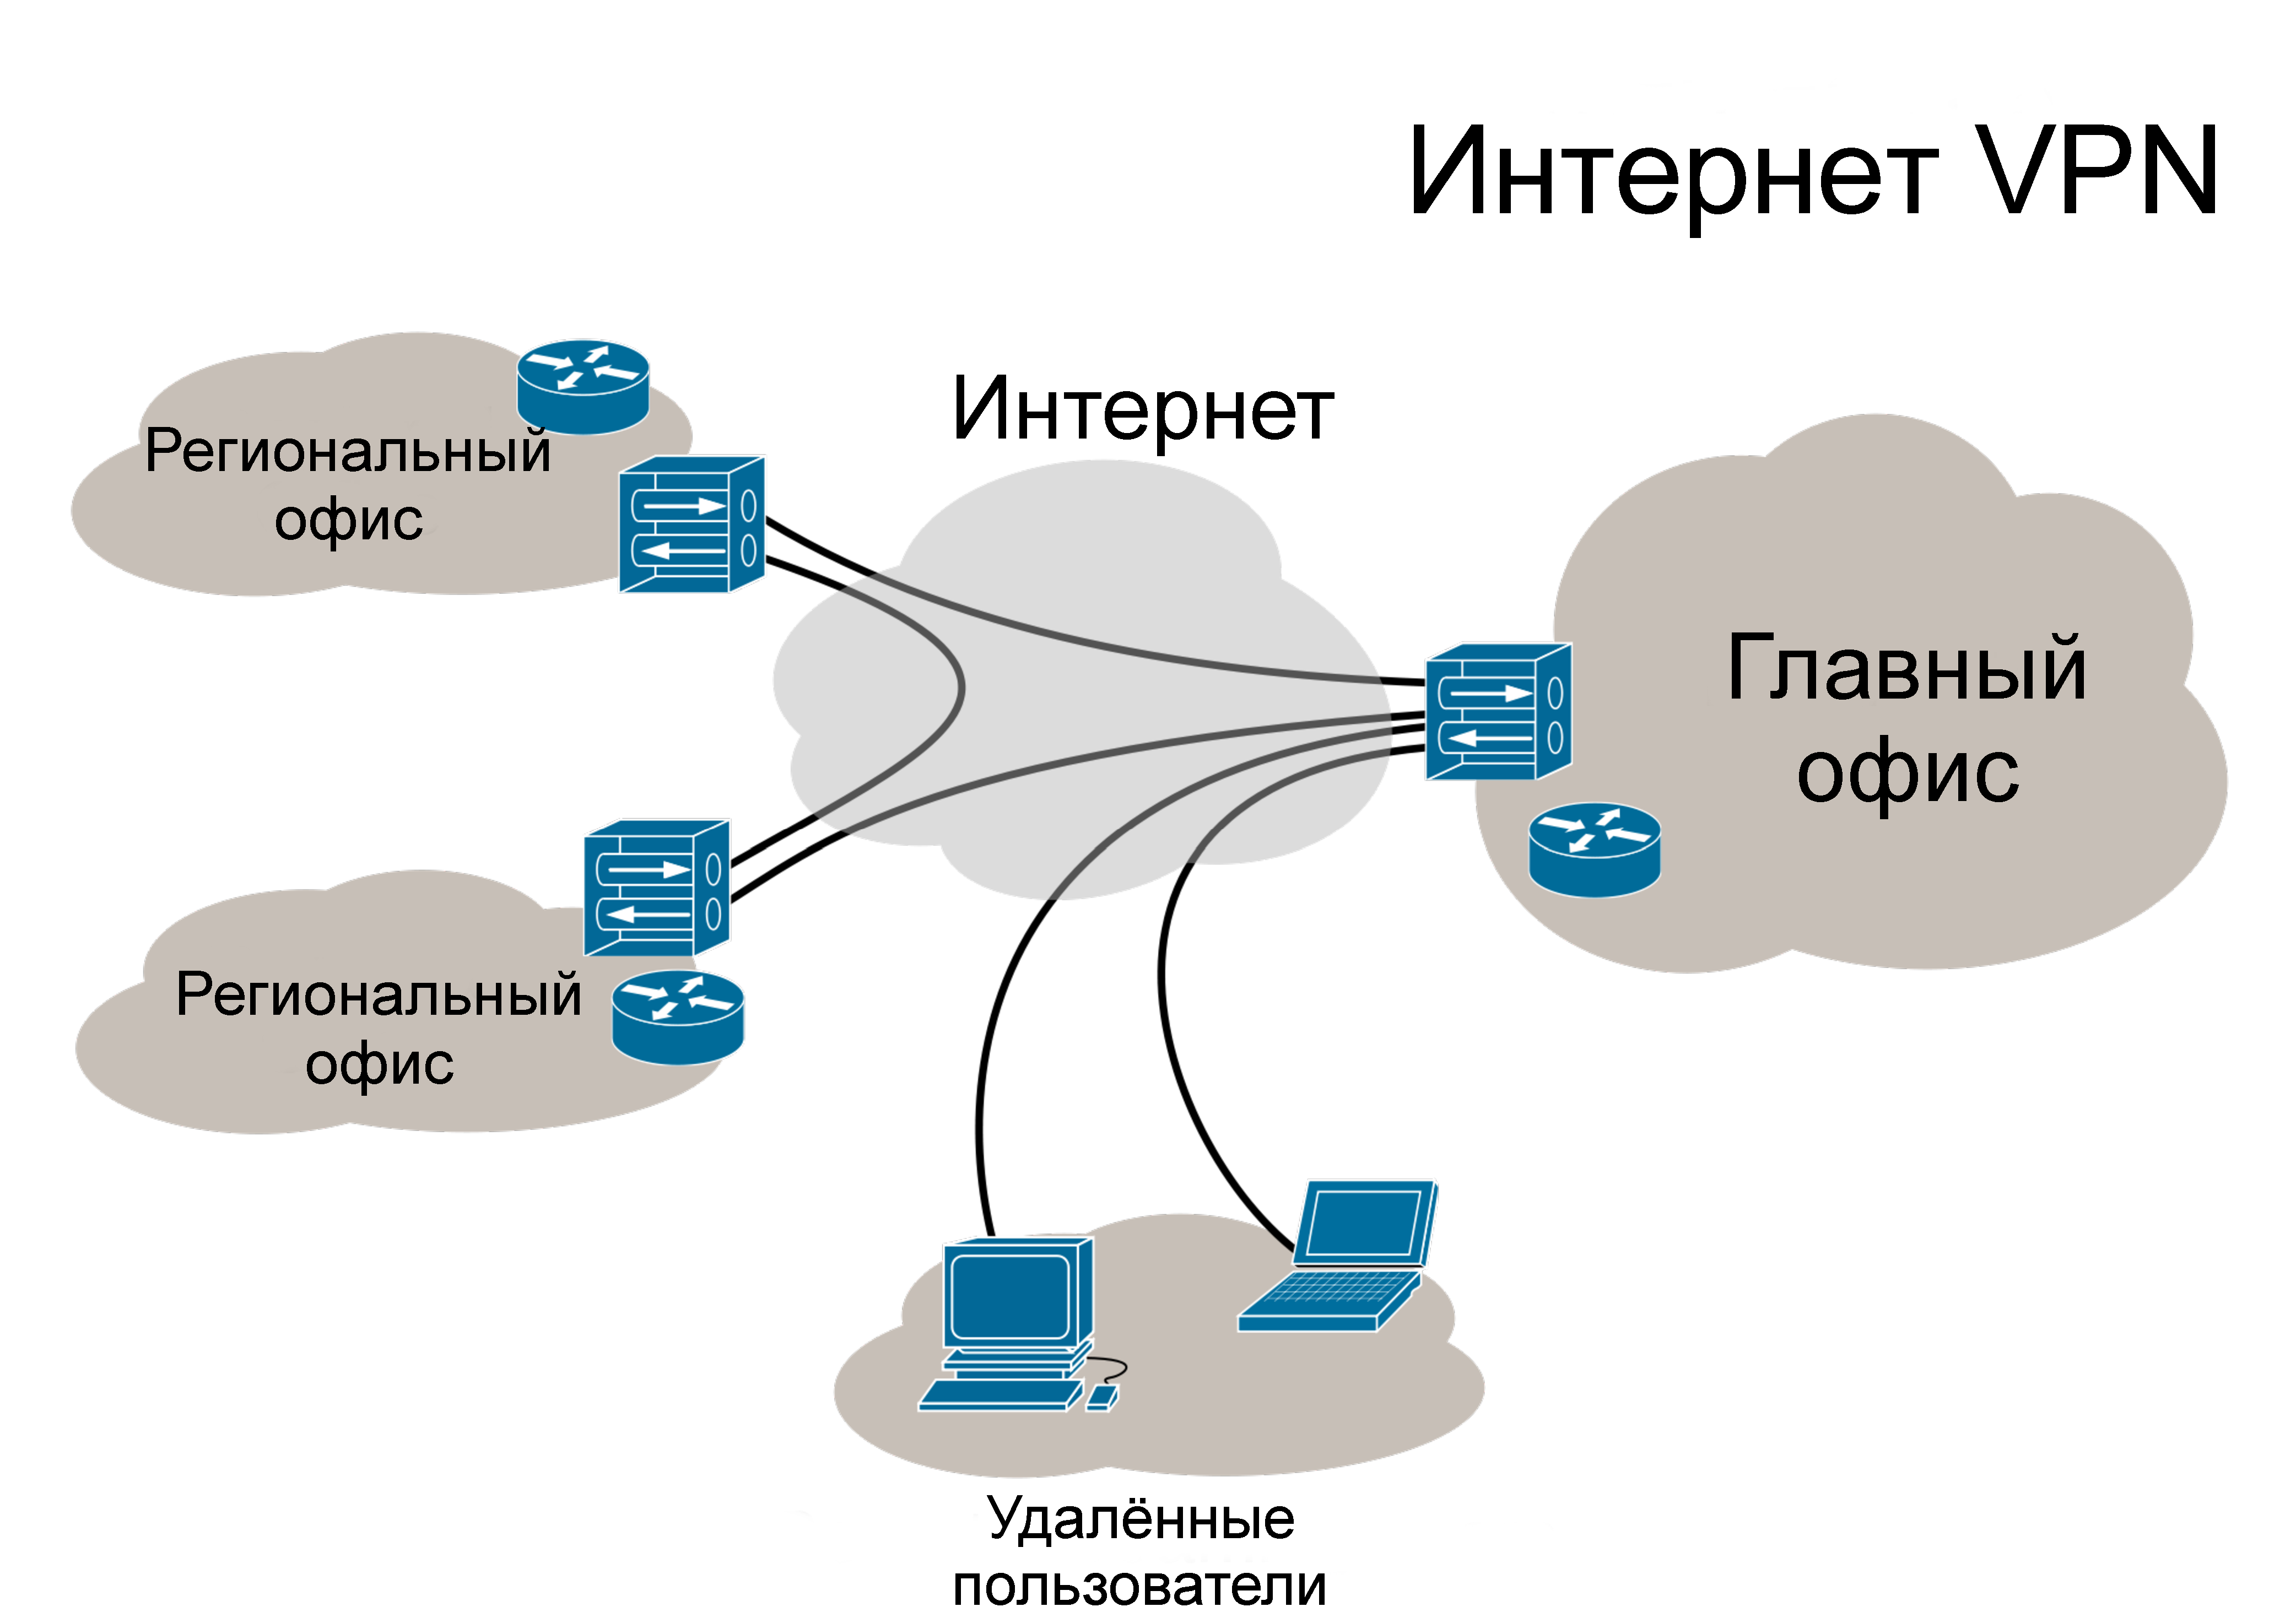
\includegraphics[width=0.7\linewidth]{vpn.pdf}
	\caption{Схема работы VPN}\label{pic:vpn}
\end{figure}

Прежде чем запускать контейнер нужно убедиться, что модуль TUN загружен:
\begin{lstlisting}
# lsmod | grep tun
\end{lstlisting}

В случае, если он не загружен, загрузить его можно следующей командой:
\begin{lstlisting}
# modprobe tun
\end{lstlisting}
\begin{lstlisting}
# lsmod | grep tun
tun     1957    0
\end{lstlisting}

Разрешаем использовать устройство TUN контейнеру:
\begin{lstlisting}
# vzctl set 101 --devnodes net/tun:rw --save
CT configuration saved to /etc/vz/conf/101.conf
\end{lstlisting}
\begin{lstlisting}
# vzctl set 101 --devices c:10:200:rw --save
CT configuration saved to /etc/vz/conf/101.conf
\end{lstlisting}
\begin{lstlisting}
# vzctl set 101 --capability net_admin:on --save
CT configuration saved to /etc/vz/conf/101.conf
\end{lstlisting}

Запускаем контейнер:
\begin{lstlisting}
# vzctl start 101
Starting container...
...
Container start in progress...
\end{lstlisting}

Создаем в контейнере собственное устройство TUN:
\begin{lstlisting}
# vzctl exec 101 mkdir -p /dev/net
# vzctl exec 101 mknod /dev/net/tun c 10 200
# vzctl exec 101 chmod 600 /dev/net/tun
\end{lstlisting}

На этом настройка устройства TUN окончена.
Далее необходимо установить ПО для работы с VPN.
Например одну из программ:
\begin{itemize}
    \item tinc (\url{http://tinc-vpn.org});
    \item OpenVPN (\url{http://openvpn.net});
    \item VTun (\url{http://vtun.sourceforge.net}).
\end{itemize}

Для установки сервера OpenVPN, можно обратиться к официальной документации, расположенной по адресу: \url{http://openvpn.net/index.php/open-source/documentation.html}

\subsection{IPTables}
Для того, чтобы в контейнере могли использоваться собственные правила IPTables, необходимо убедиться что в файле \texttt{/etc/vz/vz.conf} присутствует строка:
\begin{lstlisting}
IPTABLES="ipt_owner ipt_REDIRECT ipt_recent ip_tables iptable_filter iptable_mangle ipt_limit ipt_multiport ipt_tos ipt_TOS ipt_REJECT ipt_TCPMSS ipt_tcpmss ipt_ttl ipt_LOG ipt_length ip_conntrack ip_conntrack_ftp ipt_state iptable_nat ip_nat_ftp"
\end{lstlisting}

Если же строки нет, то ее надо добавить и перезагрузить контейнер для применения настроек:
\begin{lstlisting}
# vim /etc/vz/vz.conf
\end{lstlisting}
\begin{lstlisting}
# vzctl restart 101
\end{lstlisting}

\subsection{FUSE}
FUSE (Filesystem in Userspace) "--- модуль Linux-ядра, позволяющий создавать виртуальные файловые системы.
FUSE может пригодится, например при монтировании Яндекс.Диска или других виртуальных файловых систем.

Для того, чтобы для контейнеров был доступен FUSE, его необходимо включить на хост-ноде:
\begin{lstlisting}
# modprobe fuse
\end{lstlisting}

Проверить, что модуль успешно подключен:
\begin{lstlisting}
# lsmod | grep fuse
fuse  92980  54
\end{lstlisting}

Также необходимо добавить автозагрузку модуля при перезапуске хост-ноды:
\begin{lstlisting}
# vim /etc/rc.local
#!/bin/sh
...
modprobe fuse
\end{lstlisting}

Проброс FUSE для контейнера 101:
\begin{lstlisting}
# vzctl stop 101
# vzctl set 101 --devnodes fuse:rw --save
# vzctl set 101 --devices c:10:229:rw --save
# vzctl start 101
\end{lstlisting}

В контейнере проверяем, пробросилось ли устройство:
\begin{lstlisting}
[root@stud1 /]# ls /dev/fuse
/dev/fuse
\end{lstlisting}

Пример подключения Яндекс.Диска:
\begin{lstlisting}
# mount -t davfs https://webdav.yandex.ru /mnt/yandex.disk/
Please enter the username to authenticate with server
https://webdav.yandex.ru or hit enter for none.
  Username: username
Please enter the password to authenticate user username with server
https://webdav.yandex.ru or hit enter for none.
  Password:  pass
\end{lstlisting}

\clearpage
